% !TEX root = ../main.tex

\chapter{Evaluation of the QMC X-ray Simulation Framework}
\label{chapter11}

This final chapter provides an evaluation of the simulation framework developed
in Chapter~\ref{chapter9} and Chapter~\ref{chapter10}. The focus is on assessing
the impact of different sampling strategies --- classical \acf{mc} and the
\acf{qmc} methods based on Halton and Sobol' low-discrepancy sequences --- on
the quality of simulated X-ray images. The chapter first outlines the experimental setup, then introduces the
evaluation metrics and finally presents
the evaluation of both primary and scattered intensities. A concluding section
summarizes the findings and highlights promising directions for future research.


\section{Experimental Setup}
\label{sec:experimental_setup}

All evaluations were carried out using the simulation framework introduced in
Chapter~\ref{chapter9}. The experiments were configured via YAML-based setup
files to ensure reproducibility. The YAML-based setup is provided here to ensure that the experiments can be exactly reproduced by the reader.

For the evaluation, two main scene setups were considered: To determine how evenly distributed the simulated photons are, a homogeneous phantom was used. To evaluate the accuracy of scatter estimation, a phantom with an embedded high-density object was employed. The following sections detail the configuration of these setups. 

\subsection{Homogeneous Water Wall Phantom}

The first evaluation setup consists of a homogeneous water wall phantom, which
is used to assess the uniformity of primary and scattered intensities across the
detector. The configuration setup is described in the following.

\paragraph{Phantom.}\ \\
The phantom object is a \texttt{WaterWall}. The
entry \texttt{shape: [200, 200, 1200]} specifies the \emph{number of voxels}
along $(x,y,z)$. With cubic voxels of size \texttt{voxel\_size}
$=0.1\,\mathrm{cm}=1\,\mathrm{mm}$, the physical dimensions of the voxel grid
are $200\,\mathrm{mm} \times 200\,\mathrm{mm} \times 1200\,\mathrm{mm}$ (i.e.,
$20\,\mathrm{cm} \times 20\,\mathrm{cm} \times 120\,\mathrm{cm}$). The wall
thickness was set to \texttt{wall\_thickness} $=7.0\,\mathrm{cm}$, such that the
relevant beam--phantom interaction corresponds to a water layer of
$7\,\mathrm{cm}$.  
The detector is placed directly behind the phantom, with
\texttt{detector\_distance} $=1.0$ corresponding to a $1\,\mathrm{cm}$ gap
between the water wall and the detector plane.

\begin{lstlisting}
PHANTOM:
    object: WaterWall
    shape: [200, 200, 1200]
    wall_thickness: 7.0
    voxel_size: 0.1
    detector_distance: 1.0
\end{lstlisting}

A visualization of the scene setup is shown in Figure~\ref{fig:water_wall_scene}.

\begin{figure}[H]
\centering
\resizebox{\linewidth}{!}{%
\begin{tikzpicture}[x=1cm,y=1cm,>=Latex]

    % Styles
    \tikzstyle{plane}=[fill=gray!15,draw=black,thick]
    \tikzstyle{slab}=[fill=blue!10,draw=blue!60,thick]
    \tikzstyle{detector}=[fill=green!10,draw=green!60!black,thick]
    \tikzstyle{dimarrow}=[-{Stealth[length=3mm,width=2mm]}]
    \tikzstyle{note}=[font=\small]

    % Coordinates (x axis is beam direction →)
    \def\ys{-2}
    \def\yh{ 2}

    % Water wall: thickness 7 cm, from x=5 to x=12
    \def\xwallL{5}
    \def\xwallR{12}
    \def\wallThick{7} % cm

    % Detector plane: 1 cm gap after wall
    \def\gap{1.0}     % cm  <<< changed from 0.1 to 1.0
    \def\xdet{\xwallR+\gap}
    \def\detW{0.2}    % visual thickness of detector

    % --- Draw elements ---
    % Source plane (ExtendedSource)
    \draw[plane] (0,\ys) rectangle (0.2,\yh);
    \node[note, align=center] at (0.1,\yh+.4) {Extended source plane};

    % Emission arrows perpendicular to source plane (parallel beam)
    \foreach \yy in {-1.8,-0.9,0,0.9,1.8}{
        \draw[->,thick] (0.25,\yy) -- ++(1.2,0);
    }
    \node[note,align=left,anchor=north west] at (0.35,-2.2)
        {Emission direction};

    % Water wall slab
    \draw[slab] (\xwallL,\ys) rectangle (\xwallR,\yh);
    \node[note,align=center] at ({(\xwallL+\xwallR)/2},\yh+0.4)
        {Water wall};
    % Thickness dimension (7 cm)
    \draw (\xwallL,\ys-0.6) -- node[below=2pt] {\small $7\,\mathrm{cm}$} (\xwallR,\ys-0.6);
    \draw[thick] (\xwallL,\ys-0.4) -- (\xwallL,\ys-0.8);
    \draw[thick] (\xwallR,\ys-0.4) -- (\xwallR,\ys-0.8);

    % Detector plane with 1 cm gap to wall
    \draw[detector] (\xdet,\ys) rectangle (\xdet+\detW,\yh);
    \node[note,align=center] at (\xdet+\detW/2,\yh+.4) {Detector plane};

    % Gap annotation (1 cm)
    \draw (\xwallR,\ys-.6) -- node[below=2pt] {\small $1\,\mathrm{cm}$} (\xdet,\ys-.6);
    \draw[thick] (\xwallR,\ys-.4) -- (\xwallR,\ys-.8);
    \draw[thick] (\xdet,\ys-.4) -- (\xdet,\ys-.8);

\end{tikzpicture}
}
\caption{Schematic setup of the Water Wall Scene.}
\label{fig:water_wall_scene}
\end{figure}


\paragraph{Photon Sampling.}  \ \\
The photon generation and transport were configured as follows:

\begin{lstlisting}
SAMPLER:
    sampling_strategy: "Halton"
    num_photons: 3e6
    num_scatters: 20
    batch_size: 1e5
\end{lstlisting}

Here, \texttt{sampling\_strategy} determines the type of sequence used to
generate random numbers. The options considered were \texttt{"MC"}
(pseudo-random Monte Carlo), \texttt{"Halton"} (Halton low-discrepancy
sequence), and \texttt{"Sobol"} (Sobol' low-discrepancy sequence).  
The total number of simulated photons \texttt{num\_photons} was varied between
$0.5 \times 10^6$ and $5 \times 10^6$ in steps of $0.5 \times 10^6$.  
The parameter \texttt{num\_scatters} defines the maximum number of scattering
events per photon for the forced fixed detection algorithm (see Chapter
\ref{chapter10}). The \texttt{batch\_size} controls the number of photons
processed per iteration of the algorithm to avoid excessive memory usage
($10^5$). The photons are emitted from an extended quadratic source spans across
the cross-section of the $200\times 200\times 1200$ scene. The emission
direction is set to be perpendicular to the plane. This corresponds to the
\emph{extended source model} as described in
Section~\ref{sec:photon_position_direction}.

This setup ensures that the evaluation systematically compares the three
sampling strategies under increasing photon counts, while keeping the geometry
and transport parameters fixed.


\subsection{Bone-in-Water Phantom}

The second evaluation setup consists of a water wall phantom with embedded bone
structures. This configuration is used to assess the robustness of scatter
estimation in the presence of high-density inclusions, which introduce stronger
attenuation and more complex scattering behaviour compared to the homogeneous
case. The configuration is as follows:

\paragraph{Phantom.}\ \\
The phantom object is a \texttt{BoneWaterWall}. The entry \texttt{shape: [200,
200, 1200]} specifies the \emph{number of voxels} along $(x,y,z)$. With cubic
voxels of size \texttt{voxel\_size} $=0.1\,\mathrm{cm}=1\,\mathrm{mm}$, the
physical dimensions of the voxel grid are $200\,\mathrm{mm} \times
200\,\mathrm{mm} \times 1200\,\mathrm{mm}$ (i.e., $20\,\mathrm{cm} \times
20\,\mathrm{cm} \times 120\,\mathrm{cm}$). The wall thickness was again set to
\texttt{wall\_thickness} $=7.0\,\mathrm{cm}$, ensuring comparability with the
homogeneous water wall setup. The detector is placed directly behind the
phantom, with \texttt{detector\_distance} $=1.0$ corresponding to a
$1\,\mathrm{cm}$ gap between phantom and detector plane.

In contrast to the homogeneous water wall, this phantom includes
\texttt{n\_bones} $=3$ bone structures embedded within the water wall. The
parameter \texttt{wall\_material\_id} $=1$ specifies water as the background
material, while \texttt{bone\_material\_id} $=2$ assigns bone as the material
for the inclusions. The material-id does not only reference a material, but also
the typical density of the material, which is used to compute the attenuation
coefficients. This setup introduces regions of high attenuation and anisotropic
scattering, thereby providing a more challenging and realistic test for the
evaluation of quasi-Monte Carlo methods in scatter estimation.

\begin{lstlisting}
PHANTOM:
    object: BoneWaterWall
    shape: [200, 200, 1200]
    wall_thickness: 7.0
    voxel_size: 0.1
    detector_distance: 1.0

    n_bones: 3
    wall_material_id: 1
    bone_material_id: 2
\end{lstlisting}

\paragraph{Photon Sampling.}  \ \\
The photon generation and transport were configured mostly identically to the
homogeneous water wall setup. The only difference is that instead of the extended source model, the point source model is used here, where the source point is set to be at the center of the opposite side of the detector. This corresponds to a typical cone-beam CT setup.

Figure~\ref{fig:bone_water_cone_beam} illustrates the scene setup with the point
source emitting cone-beam rays through the water wall containing bone cylinders.

\begin{figure}[H]
\centering
\resizebox{\linewidth}{!}{%
\begin{tikzpicture}[x=1cm,y=1cm,>=Latex]

    % Styles
    \tikzstyle{source}=[fill=gray!30,draw=black,thick]
    \tikzstyle{slab}=[fill=blue!8,draw=blue!60,thick]
    \tikzstyle{bone}=[fill=orange!60,draw=orange!80!black,thick]
    \tikzstyle{detector}=[fill=green!10,draw=green!60!black,thick]
    \tikzstyle{dimline}=[-{Stealth[length=3mm,width=2mm]}]
    \tikzstyle{note}=[font=\small]

    % --- Geometry parameters ---
    % y-extent for drawing
    \def\ymin{-3}
    \def\ymax{ 3}

    % Source at origin
    \coordinate (S) at (0,0);

    % Water wall: thickness 7 cm, from x=6 to x=13
    \def\xwallL{6}
    \def\xwallR{13}

    % Detector plane: 1 cm gap after wall
    \def\gap{1.0}   % cm
    \def\xdet{\xwallR+\gap}  % = 14
    \def\detW{0.25} % visual thickness

    % --- Draw elements ---
    % Source point (point source)
    \draw[source] (S) circle (0.08);
    \node[note,anchor=south] at ([yshift=0.25cm]S) {Point source};

    % Detector plane
    \draw[detector] (\xdet,\ymin) rectangle (\xdet+\detW,\ymax);
    \node[note,align=center] at (\xdet+\detW/2,\ymax+0.4) {Detector plane};

    % Water wall slab
    \draw[slab] (\xwallL,\ymin) rectangle (\xwallR,\ymax);
    \node[note] at ({(\xwallL+\xwallR)/2},\ymax+0.4) {Water wall};
    % ----------
    \draw[fill=orange!60,draw=none] ({\xwallL+0.7},-1.225) rectangle ({\xwallR-0.7},-2.325);
    \draw[draw=orange!80!black,thick] ({\xwallL+0.7},-2.325) -- ({\xwallR-0.7},-2.325);
    \draw[draw=orange!80!black,thick] ({\xwallL+0.7},-1.225) -- ({\xwallR-0.7},-1.225);
    \draw[white, fill=white] ({\xwallL+0.7},-1.775) ellipse [x radius=0.25, y radius=0.55];
    \draw[bone,opacity=0.7] ({\xwallL+0.7},-1.775) ellipse [x radius=0.25, y radius=0.55];
    \draw[draw=orange!60] ({\xwallR-0.7},-1.775) -- ({\xwallR-0.7},-1.225);
    \draw[bone,domain=-90:90] plot ({\xwallR-0.7 + 0.25*cos(\x)}, {-1.775 + 0.55*sin(\x)});
    \node[note,align=center] at ({(\xwallL+\xwallR)/2},\ymin-0.6) {Bone cylinder};


    % ----------
    \draw[fill=orange!60,draw=none] ({\xwallL+0.7},0.55) rectangle ({\xwallR-0.7},-0.55);
    \draw[draw=orange!80!black,thick] ({\xwallL+0.7},-0.55) -- ({\xwallR-0.7},-0.55);
    \draw[draw=orange!80!black,thick] ({\xwallL+0.7},0.55) -- ({\xwallR-0.7},0.55);
    \draw[white, fill=white] ({\xwallL+0.7},0) ellipse [x radius=0.25, y radius=0.55];
    \draw[bone,opacity=0.7] ({\xwallL+0.7},0) ellipse [x radius=0.25, y radius=0.55];
    \draw[draw=orange!60] ({\xwallR-0.7},0) -- ({\xwallR-0.7},0.55);
    \draw[bone,domain=-90:90] plot ({\xwallR-0.7 + 0.25*cos(\x)}, {0 + 0.55*sin(\x)});
    \node[note,align=center] at ({(\xwallL+\xwallR)/2},\ymin-0.6) {Bone cylinder};


    % ----------
    \draw[fill=orange!60,draw=none] ({\xwallL+0.7},2.325) rectangle ({\xwallR-0.7},1.225);
    \draw[draw=orange!80!black,thick] ({\xwallL+0.7},1.225) -- ({\xwallR-0.7},1.225);
    \draw[draw=orange!80!black,thick] ({\xwallL+0.7},2.325) -- ({\xwallR-0.7},2.325);
    \draw[white, fill=white] ({\xwallL+0.7},1.775) ellipse [x radius=0.25, y radius=0.55];
    \draw[bone,opacity=0.7] ({\xwallL+0.7},1.775) ellipse [x radius=0.25, y radius=0.55];
    \draw[draw=orange!60] ({\xwallR-0.7},1.775) -- ({\xwallR-0.7},2.325);
    \draw[bone,domain=-90:90] plot ({\xwallR-0.7 + 0.25*cos(\x)}, {1.775 + 0.55*sin(\x)});
    \node[note,align=center] at ({(\xwallL+\xwallR)/2},\ymin-0.6) {Bone cylinder};

    

    % Cone-beam rays from source to detector (sample a few points across the detector)
    \draw[fill=yellow,opacity=0.3] (S) -- (\xdet,\ymin) -- (\xdet,\ymax) -- cycle;

    \node[note,align=left] at (1.3,2.4) {Divergent rays (cone-beam)};

    % --- Dimensions ---
    % Wall thickness (7 cm)
    \draw[dimline] (\xwallL,\ymin-0.9) -- node[below=2pt] {\small $7\,\mathrm{cm}$} (\xwallR,\ymin-0.9);
    \draw[thick] (\xwallL,\ymin-0.7) -- (\xwallL,\ymin-1.1);
    \draw[thick] (\xwallR,\ymin-0.7) -- (\xwallR,\ymin-1.1);

    % Detector gap (1 cm)
    \draw[dimline] (\xwallR,\ymin-1.8) -- node[below=2pt] {\small $1\,\mathrm{cm}$} (\xdet,\ymin-1.8);
    \draw[thick] (\xwallR,\ymin-1.6) -- (\xwallR,\ymin-2.0);
    \draw[thick] (\xdet,\ymin-1.6) -- (\xdet,\ymin-2.0);

\end{tikzpicture}
}
\caption{Point source emitting cone-beam rays through a water wall containing bone cylinders.}
\label{fig:bone_water_cone_beam}
\end{figure}




\section{Evaluation Metric}
\label{sec:evaluation_metrics}

To introduce the metric used for evaluation of the X-ray simulation results,
the scene is chosen to be the simpler water wall phantom, where one expects the primary
and scattered intensities to be spatially uniform across the detector. This
allows for an evaluation of how evenly distributed the simulated photon
intensities are. 

The evaluation of the simulation results is based on the image quality metric
\emph{noise}. In contrast to repeated simulations, here a single simulation with
$N$ photons is performed and the resulting image is analysed over all detector
pixels. Let $\Omega$ denote the set of detector pixels and $|\Omega|$ its
cardinality.

\begin{definition}[Noise]\ \\
Let $I(p)$ denote the simulated intensity at pixel $p \in \Omega$, and let
\[
    \bar{I} = \frac{1}{|\Omega|} \sum_{p \in \Omega} I(p)
\]
be the mean intensity across all pixels. The \emph{noise} is defined as the
standard deviation of the pixel intensities,
\[
    \sigma \;=\; 
    \sqrt{\frac{1}{|\Omega|}\sum_{p \in \Omega} \bigl(I(p) - \bar{I}\bigr)^2}.
\]
It quantifies the variability of the simulated intensities across the detector
plane.
\end{definition}

Runtime was deliberately not chosen as an evaluation metric. The computational
time depends strongly on the chosen phantom, the complexity of the scene, and
the employed hardware. Instead, the number of simulated photons $N$ is used as
the controlling parameter, as it provides a scene-independent measure of the
simulation effort and ensures comparability across different experiments.


\section{Evaluation Results}
\subsection{Primary Intensities}

Although expected primary intensities can be directly computed by tracing only
the straight rays from the source to each detector pixel and computing their
attenuation along the way, for physically correct photon simulations they arise
naturally whether wanted or not. Primary intensities arise from photons with
various directions and energies that reach the detector without any interaction.
This leads to a certain amount of noise in the primary intensities, which can be
reduced by increasing the number of simulated photons. As the following
experiments will show, the sampling strategy has a significant impact on the
noise level of the primary intensities.

\begin{figure}[H]
    \centering
    \begin{subfigure}[b]{0.49\linewidth}
        \centering
        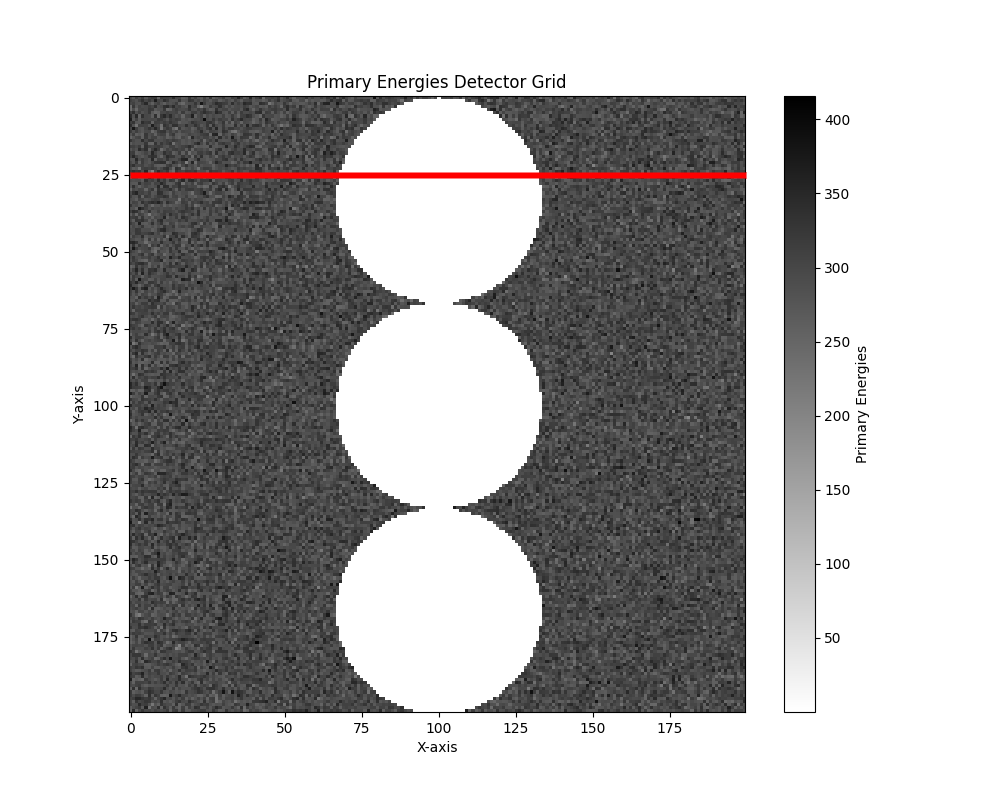
\includegraphics[width=\linewidth]{Figures/primary_boneWall_mc.png}
        \captionsetup{justification=centering}
        \caption{Monte Carlo sampling}
    \end{subfigure}
    \hfill
    \begin{subfigure}[b]{0.49\linewidth}
        \centering
        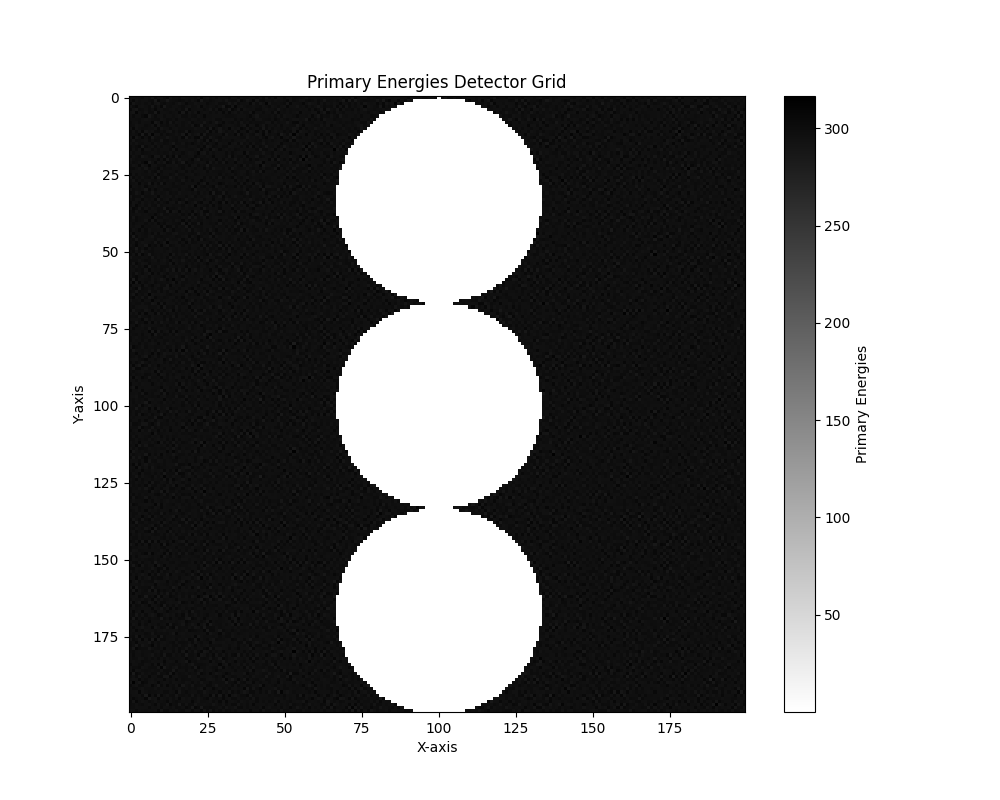
\includegraphics[width=\linewidth]{Figures/primary_boneWall_halton.png}
        \captionsetup{justification=centering}
        \caption{Halton sampling}
    \end{subfigure}
    \vspace{1em}
    \begin{subfigure}[b]{0.49\linewidth}
        \centering
        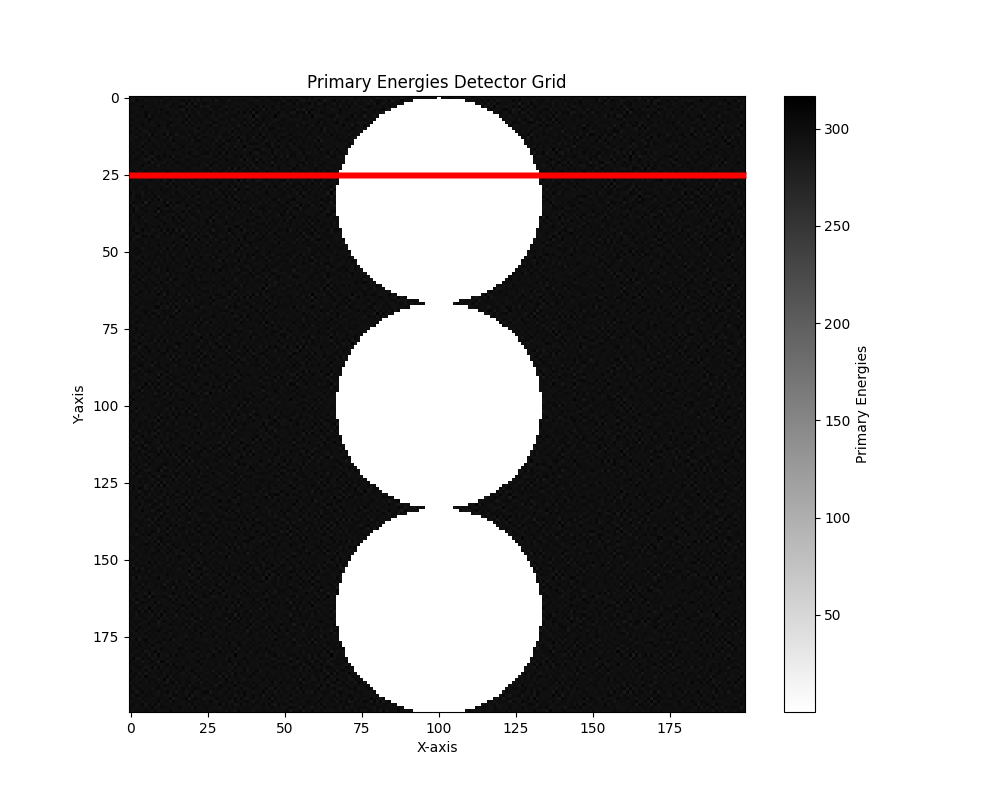
\includegraphics[width=\linewidth]{Figures/primary_boneWall_sobol.png}
        \captionsetup{justification=centering}
        \caption{Sobol' sampling}
    \end{subfigure}
    \caption{Simulated primary intensities for an X-ray of the Bone-in-Water phantom using Monte Carlo, Halton, and Sobol' sampling.}
    \label{fig:primary_intensities_comparison}
\end{figure}


Figure~\ref{fig:primary_intensities_comparison} shows the simulated primary
intensities for the Bone-in-Water phantom using different sampling startegies
for the initial direction and photon energy. Whereas the Monte Carlo result
exhibits noticable noise, the Halton and Sobol' results are significantly
smoother with almost no visible noise. In the simulation shown, $5 \times 10^6$ photons were used for each sampling strategy.

The noise can be further observed in the intensity profile along the horizontal
red line. In Figure~\ref{fig:primary_intensity_profile}, the intensity profiles
for the Sobol' and Monte Carlo sampling strategies are compared.

\begin{figure}[H]
    \centering
    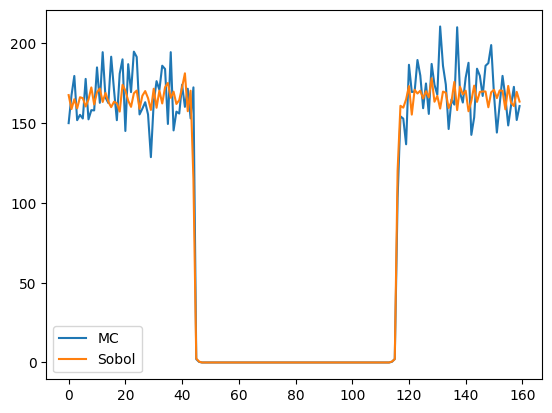
\includegraphics[width=0.6\linewidth]{Figures/primary_profile_boneWall.png}
    \caption{Intensity profile along the horizontal red line in Figure~\ref{fig:primary_intensities_comparison}.}
    \label{fig:primary_intensity_profile}
\end{figure}

To confirm these results with quantitative data, the noise levels of the primary
intensites in the homogeneous water wall phantom were measured for different
numbers of simulated photons and for each sampling strategy. The results are
summarized in Figure~\ref{fig:primary_intensity_noise}. The plot shows the noise
levels on a log-log scale. Before calculating the noise, the intensities on the
detector were normalized by the number of simulated photons to ensure
comparability.

\begin{figure}[H]
    \centering
    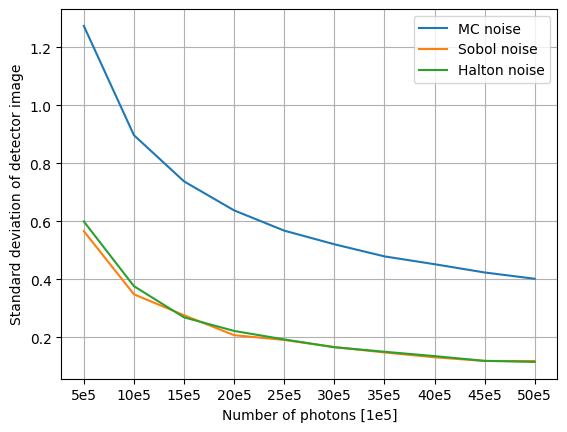
\includegraphics[width=0.6\linewidth]{Figures/primary_noise_boneWall.png}
    \caption{Plot of noise levels for primary intensities in Water-Wall Phantom for varying numbers of simulated photons.}
    \label{fig:primary_intensity_noise}
\end{figure}


\subsection{Scattered Intensities}

The chapter now turns to the evaluation of scattered intensities. Unlike primary
intensities, scattered intensities cannot be computed analytically and must be
sampled via physical simulation for good estimation. For scatter reduction, an
image with low noise is desired. Therefore, this subsection focuses on the noise
levels of the scattered intensities.

In an experimental setup, the scattering is simulated for the Bone-in-Water phantom
using the three sampling strategies. The resulting scattered intensities are
shown in Figure~\ref{fig:scattered_intensities_comparison}. Within this experiments $5 \times 10^6$ photons were simulated for each sampling strategy and the number of scattering events was set to 20.

\begin{figure}[H]
    \centering
    \begin{subfigure}[b]{0.49\linewidth}
        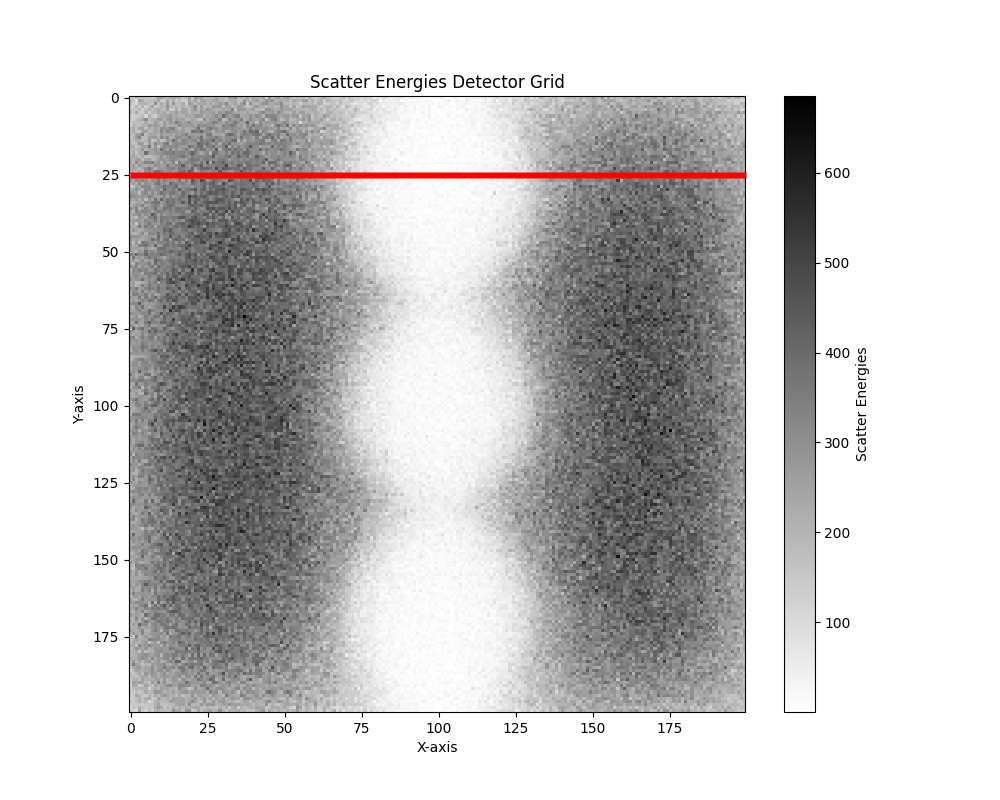
\includegraphics[width=\linewidth]{Figures/scatter_energies_mc_boneWall.png}
        \captionsetup{justification=centering}
        \caption{Monte Carlo sampling}
    \end{subfigure}
    \hfill
    \begin{subfigure}[b]{0.49\linewidth}
        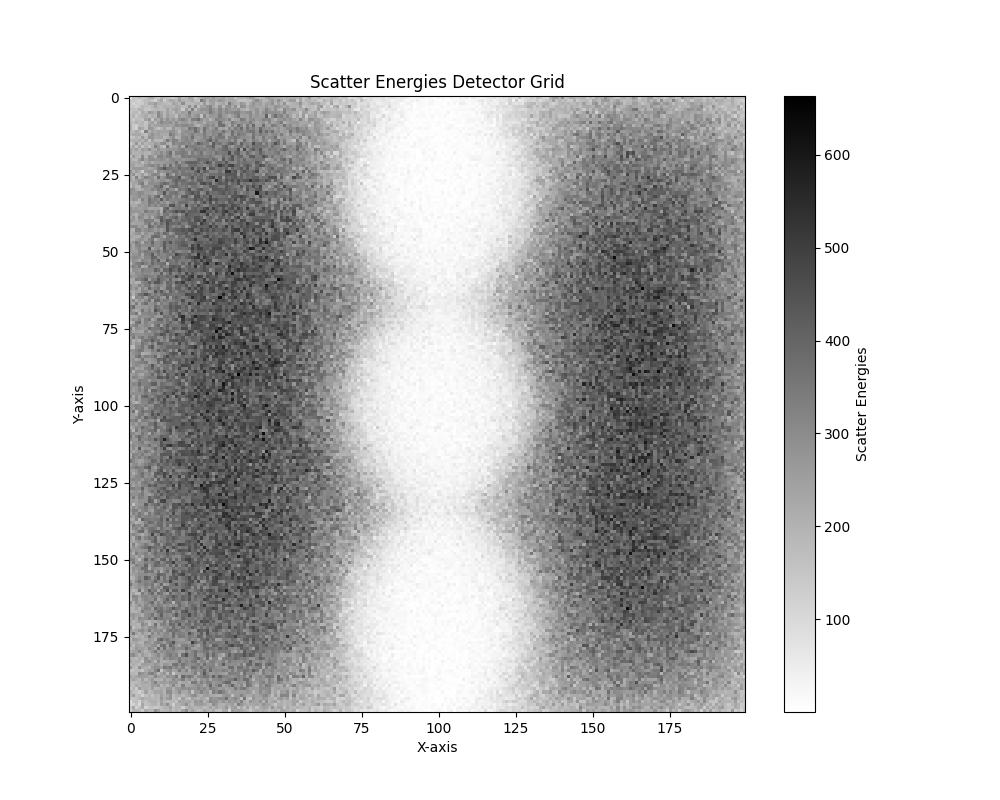
\includegraphics[width=\linewidth]{Figures/scatter_energies_halton_boneWall.png}
        \captionsetup{justification=centering}
        \caption{Halton sampling}
    \end{subfigure}
    \vspace{1em}
    \begin{subfigure}[b]{0.49\linewidth}
        \centering
        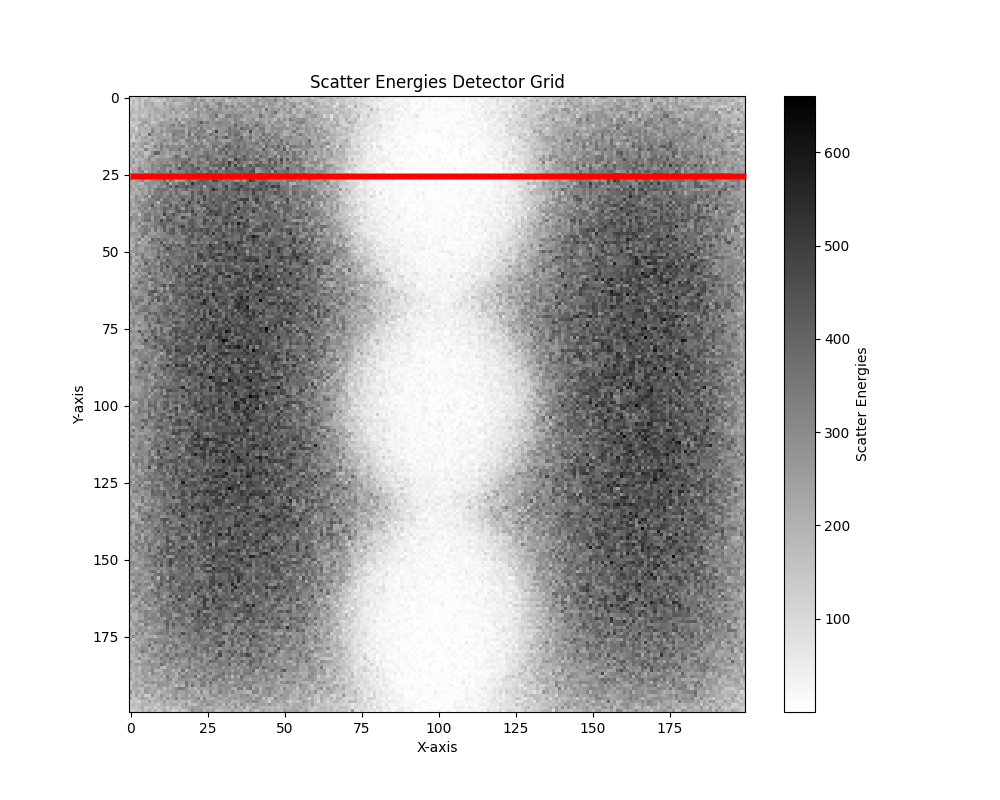
\includegraphics[width=\linewidth]{Figures/scatter_energies_sobol_boneWall.png}
        \captionsetup{justification=centering}
        \caption{Sobol' sampling}
    \end{subfigure}
    \caption{Simulated scatter intensities for an X-ray of the Bone-in-Water phantom using Monte Carlo, Halton, and Sobol' sampling.}
    \label{fig:scattered_intensities_comparison}
\end{figure}

Along the horizontal red line, the intensity profiles are extracted for the Sobol' and Monte Carlo sampling strategies, as shown in Figure~\ref{fig:scattered_intensity_profile}.

\begin{figure}[H]
    \centering
    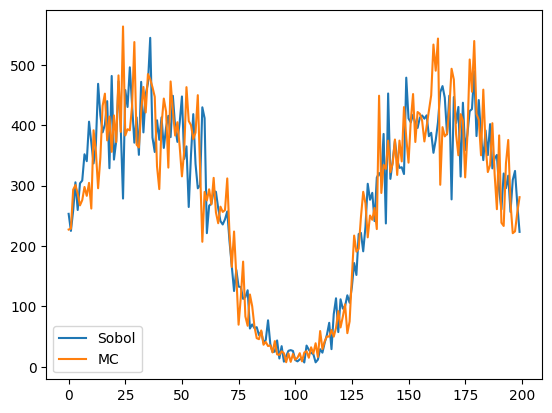
\includegraphics[width=0.7\linewidth]{Figures/scatter_energies_profile_boneWall.png}
    \caption{Intensity profile along the horizontal red line in Figure~\ref{fig:scattered_intensities_comparison}.}
    \label{fig:scattered_intensity_profile}
\end{figure}

Although the plots show a similar trend, the variance along the profile is significantly lower for the Sobol' sampling strategy. For \ac{mc} sampling, the variance shows an increase by $~7\%$ in noise. Halton sampling shows a similar performance as the quasi-random \ac{mc} sampled simulation. The forced 20 scattering events per photon do result in a 63-dimensional low-discrepancy sequence. Therefore, it was expected that the advantages of the Halton sequence would diminish, as Halton sequences are known to perform worse in higher dimensions due to correlations between the dimensions \cite{mohammed2019impact}.

\begin{table}[H]
    \centering
    \begin{tabular}{lccc}
        \toprule
        Sampling Strategy & Variance & Improvement \\
        \midrule
        Monte Carlo      & 23512    & --- \\
        Halton           & 23169    & 1\% \\
        Sobol'           & 22038    & 7\% \\
        \bottomrule
    \end{tabular}
    \caption{Variance of the intensity profile along the horizontal line for different sampling strategies. Sobol' sampling achieves a variance reduction by a factor of 6 compared to Monte Carlo.}
    \label{tab:scatter_line_variance}
\end{table}


\section{Conclusion and Future Work}

\textcolor{red}{TODO: TBD}

As the computations for scattered photons are extensive, alredy little improvements in noise levels can lead to significant reductions in computation time for real-world applications.
The chapter concludes with a summary of the evaluation findings, highlighting
the advantages and limitations of QMC-based simulation. Potential directions for
future work include extending the evaluation to more complex phantoms,
integrating additional low-discrepancy sequences, and investigating hybrid
approaches that combine QMC with variance reduction techniques.
